\subsubsection{Example}

    \begin{itemize}[noitemsep,topsep=0pt]
      \item Starting position: (-1.0, 42.0, 108.0)
      \item End position: (55.0, 43.0, 23.0) 
      \item Euclidean distance from the object: 73.50510186374821
      \item Object can be seen: False
      \item Success: False
      \item Object type: crowd
      
    \end{itemize}
    

    \begin{center}
    
\includegraphics[width=0.7\linewidth]{images/Sonnet-CityNew-FS2/20.pdf}
    \end{center}
    

    \begin{center}
    \includegraphics[width=0.7\linewidth]{images/Sonnet-CityNew-FS2/20_sit_awareness.pdf}
    \end{center}
    

    \begin{drama}
    \Character{Benchmark}{re}
    \Character{Claude 3.5 Sonnet}{gpt}
    
\respeaks: \( < \)Context\( > \)
    You are in command of a UAV, tasked with finding crowd.
\( < \)/Context\( > \) \texttt{(REST OF THE PROMPT)}
\respeaks: The object you're looking for is similar to this. This is NOT the drone's current view.
\respeaks: Image 1:
\StageDir{\re{} presents \gpt{} with a relevant image}

    \begin{center}
    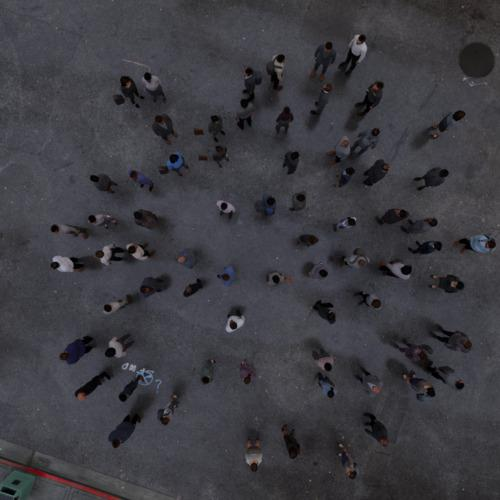
\includegraphics[width=0.5\linewidth]{images/Sonnet-CityNew-FS2/20_0.jpg}
    \end{center}
    
\respeaks: Your current altitude is 108 meters above ground level.
\respeaks: Image 2:
\StageDir{\re{} presents \gpt{} with a relevant image}

    \begin{center}
    
\includegraphics[width=0.5\linewidth]{images/Sonnet-CityNew-FS2/20_1.jpg}
    \end{center}
    
\gptspeaks: \( < \)Reasoning\( > \)From this height, I need to conduct a systematic search for a crowd gathering. I notice some potential movement near the (0, 0) coordinate. I'll move closer to that area and reduce altitude significantly to get a better view. The example shows a crowd from above, so I need to be methodical in my search while maintaining a safe distance.\( < \)/Reasoning\( > \)
\( < \)Action\( > \)(0, 0, -50)\( < \)/Action\( > \)
\respeaks: Emergency stop; you've flown too close to something and would have hit it.
\respeaks: Your current altitude is 83 meters above ground level.
\respeaks: Image 3:
\StageDir{\re{} presents \gpt{} with a relevant image}

    \begin{center}
    
\includegraphics[width=0.5\linewidth]{images/Sonnet-CityNew-FS2/20_2.jpg}
    \end{center}
    
\gptspeaks: \( < \)Reasoning\( > \)I need to be more careful about altitude changes. I see that this area appears to be indoors or covered. I should move to a different area to search for the crowd, as they're more likely to be in an open space. Let's move towards (28, 55) where there might be more open area, and maintain the current altitude for safety.\( < \)/Reasoning\( > \)
\( < \)Action\( > \)(28, 55, 0)\( < \)/Action\( > \)
\respeaks: Your current altitude is 83 meters above ground level.
\respeaks: Image 4:
\StageDir{\re{} presents \gpt{} with a relevant image}

    \begin{center}
    
\includegraphics[width=0.5\linewidth]{images/Sonnet-CityNew-FS2/20_3.jpg}
    \end{center}
    
\gptspeaks: \( < \)Reasoning\( > \)I need to expand my search area as this location shows mostly building structures. Let's move to (-55, 0) to explore the western area where there might be more open spaces that could accommodate a crowd. I'll maintain the current altitude for now until I spot a potential gathering.\( < \)/Reasoning\( > \)
\( < \)Action\( > \)(-55, 0, 0)\( < \)/Action\( > \)
\respeaks: Your current altitude is 83 meters above ground level.
\respeaks: Image 5:
\StageDir{\re{} presents \gpt{} with a relevant image}

    \begin{center}
    
\includegraphics[width=0.5\linewidth]{images/Sonnet-CityNew-FS2/20_4.jpg}
    \end{center}
    
\gptspeaks: \( < \)Reasoning\( > \)I can see an intersection and open streets below. There appears to be more visible area to the south that might be suitable for a crowd gathering. Let's move to (-55, -55) to explore that direction while maintaining our current altitude until we spot any potential gatherings.\( < \)/Reasoning\( > \)
\( < \)Action\( > \)(-55, -55, 0)\( < \)/Action\( > \)
\respeaks: Your current altitude is 83 meters above ground level.
\respeaks: Image 6:
\StageDir{\re{} presents \gpt{} with a relevant image}

    \begin{center}
    
\includegraphics[width=0.5\linewidth]{images/Sonnet-CityNew-FS2/20_5.jpg}
    \end{center}
    
\gptspeaks: \( < \)Reasoning\( > \)I see mostly streets and buildings in this area. Let's explore the eastern side of the search area where there might be open spaces or plazas. I'll move to (65, -55) to continue our systematic search while maintaining the current altitude until we spot any gatherings.\( < \)/Reasoning\( > \)
\( < \)Action\( > \)(65, -55, 0)\( < \)/Action\( > \)
\respeaks: Your current altitude is 83 meters above ground level.
\respeaks: Image 7:
\StageDir{\re{} presents \gpt{} with a relevant image}

    \begin{center}
    
\includegraphics[width=0.5\linewidth]{images/Sonnet-CityNew-FS2/20_6.jpg}
    \end{center}
    
\gptspeaks: \( < \)Reasoning\( > \)This area shows mostly rooftops with mechanical equipment. Let's check the northern area that we haven't explored yet. I'll move to (65, 55) to continue our systematic search while maintaining altitude until we find signs of a crowd gathering.\( < \)/Reasoning\( > \)
\( < \)Action\( > \)(65, 55, 0)\( < \)/Action\( > \)
\respeaks: Emergency stop; you've flown too close to something and would have hit it.
\respeaks: Your current altitude is 83 meters above ground level.
\respeaks: Image 8:
\StageDir{\re{} presents \gpt{} with a relevant image}

    \begin{center}
    
\includegraphics[width=0.5\linewidth]{images/Sonnet-CityNew-FS2/20_7.jpg}
    \end{center}
    
\gptspeaks: \( < \)Reasoning\( > \)I need to be more careful about obstacles. This appears to be an indoor or covered area, which isn't suitable for crowd gatherings. Let's move back towards (0, -55) where there might be more open space, and stay at our current altitude for safety.\( < \)/Reasoning\( > \)
\( < \)Action\( > \)(0, -55, 0)\( < \)/Action\( > \)
\respeaks: Your current altitude is 83 meters above ground level.
\respeaks: Image 9:
\StageDir{\re{} presents \gpt{} with a relevant image}

    \begin{center}
    
\includegraphics[width=0.5\linewidth]{images/Sonnet-CityNew-FS2/20_8.jpg}
    \end{center}
    
\gptspeaks: \( < \)Reasoning\( > \)I'm still seeing mostly rooftop structures. Since we've explored several areas without finding the crowd, let's try moving to (0, 55) to check the northern open areas. I'll maintain the current altitude until we spot potential gathering spaces.\( < \)/Reasoning\( > \)
\( < \)Action\( > \)(0, 55, 0)\( < \)/Action\( > \)
\respeaks: Your current altitude is 83 meters above ground level.
\respeaks: Image 10:
\StageDir{\re{} presents \gpt{} with a relevant image}

    \begin{center}
    
\includegraphics[width=0.5\linewidth]{images/Sonnet-CityNew-FS2/20_9.jpg}
    \end{center}
    
\gptspeaks: \( < \)Reasoning\( > \)We seem to be in some kind of covered or indoor structure. We need to get to an open area where crowds would typically gather. Let's try moving to (-55, 28) where there might be a plaza or open space, while maintaining our current altitude for safety.\( < \)/Reasoning\( > \)
\( < \)Action\( > \)(-55, 28, 0)\( < \)/Action\( > \)
\respeaks: Emergency stop; you've flown too close to something and would have hit it.
\respeaks: Your current altitude is 83 meters above ground level.
\respeaks: Image 11:
\StageDir{\re{} presents \gpt{} with a relevant image}

    \begin{center}
    
\includegraphics[width=0.5\linewidth]{images/Sonnet-CityNew-FS2/20_10.jpg}
    \end{center}
    
\gptspeaks: \( < \)Reasoning\( > \)I need to get out of this covered structure. Since we're having trouble navigating at this level, let's first gain some altitude to get a better overview of the area and avoid obstacles. I'll increase altitude by 50 meters to help identify open spaces where crowds might gather.\( < \)/Reasoning\( > \)
\( < \)Action\( > \)(0, 0, 50)\( < \)/Action\( > \)
\respeaks: Your current altitude is 133 meters above ground level.
\respeaks: Image 12:
\StageDir{\re{} presents \gpt{} with a relevant image}

    \begin{center}
    
\includegraphics[width=0.5\linewidth]{images/Sonnet-CityNew-FS2/20_11.jpg}
    \end{center}
    
\gptspeaks: \( < \)Reasoning\( > \)From this higher vantage point, I can see what appears to be an open area to the northwest (-89, 44). That looks like the kind of space where a crowd might gather. Let's move there to investigate while maintaining this safer altitude before making any descent.\( < \)/Reasoning\( > \)
\( < \)Action\( > \)(-89, 44, 0)\( < \)/Action\( > \)
\respeaks: Your current altitude is 133 meters above ground level.
\respeaks: Image 13:
\StageDir{\re{} presents \gpt{} with a relevant image}

    \begin{center}
    
\includegraphics[width=0.5\linewidth]{images/Sonnet-CityNew-FS2/20_12.jpg}
    \end{center}
    
\gptspeaks: \( < \)Reasoning\( > \)I can see a large open area in the southeast quadrant of the image. Let's move to (89, -89) to investigate that space. From this altitude, we have a good overview but we'll need to descend once we spot any potential crowd gatherings.\( < \)/Reasoning\( > \)
\( < \)Action\( > \)(89, -89, 0)\( < \)/Action\( > \)
\respeaks: Your current altitude is 133 meters above ground level.
\respeaks: Image 14:
\StageDir{\re{} presents \gpt{} with a relevant image}

    \begin{center}
    
\includegraphics[width=0.5\linewidth]{images/Sonnet-CityNew-FS2/20_13.jpg}
    \end{center}
    
\gptspeaks: \( < \)Reasoning\( > \)I'm seeing what appears to be the rooftop of a building with mechanical equipment. Looking at the entire search pattern so far, we haven't thoroughly checked the northeastern area. Let's move to (89, 89) to explore that sector while maintaining this altitude for a good overview.\( < \)/Reasoning\( > \)
\( < \)Action\( > \)(89, 89, 0)\( < \)/Action\( > \)
\respeaks: Your current altitude is 133 meters above ground level.
\respeaks: Image 15:
\StageDir{\re{} presents \gpt{} with a relevant image}

    \begin{center}
    
\includegraphics[width=0.5\linewidth]{images/Sonnet-CityNew-FS2/20_14.jpg}
    \end{center}
    
\gptspeaks: \( < \)Reasoning\( > \)I see streets and buildings but no crowd gatherings yet. Let's move to (0, 89) to explore the northern area more thoroughly. We've covered most other directions, so this is one of our remaining unexplored areas that could potentially have open spaces suitable for crowds.\( < \)/Reasoning\( > \)
\( < \)Action\( > \)(0, 89, 0)\( < \)/Action\( > \)
\respeaks: Your current altitude is 133 meters above ground level.
\respeaks: Image 16:
\StageDir{\re{} presents \gpt{} with a relevant image}

    \begin{center}
    
\includegraphics[width=0.5\linewidth]{images/Sonnet-CityNew-FS2/20_15.jpg}
    \end{center}
    
\gptspeaks: \( < \)Reasoning\( > \)From this vantage point, I can see what appears to be a triangular open space or plaza. Let's move to (-44, 44) to get a better view of this area, and then we can consider descending if we spot any crowd gatherings. We need to be methodical as we haven't found our target yet.\( < \)/Reasoning\( > \)
\( < \)Action\( > \)(-44, 44, 0)\( < \)/Action\( > \)
\respeaks: This command would cause you to fly out of the search area's bounds. You can't fly further than 108.0 meters from the starting point in any axis.
\gptspeaks: \( < \)Reasoning\( > \)I apologize for trying to exceed the search bounds. Let's adjust our strategy. Since we're at 133 meters height and haven't found the crowd yet, we should try descending a bit in a central location to get a clearer view. I'll move to (0, 0) and reduce altitude to get a better look at the ground level while staying within bounds.\( < \)/Reasoning\( > \)
\( < \)Action\( > \)(0, 0, -30)\( < \)/Action\( > \)
\respeaks: Your current altitude is 103 meters above ground level.
\respeaks: Image 17:
\StageDir{\re{} presents \gpt{} with a relevant image}

    \begin{center}
    
\includegraphics[width=0.5\linewidth]{images/Sonnet-CityNew-FS2/20_16.jpg}
    \end{center}
    
\gptspeaks: \( < \)Reasoning\( > \)I see we're still quite high up and looking at mostly building structures. Let's check the southern area at (0, -69) and continue descending to get closer to ground level where crowds would be. We need to find open spaces at street level.\( < \)/Reasoning\( > \)
\( < \)Action\( > \)(0, -69, -20)\( < \)/Action\( > \)
\respeaks: Your current altitude is 83 meters above ground level.
\respeaks: Image 18:
\StageDir{\re{} presents \gpt{} with a relevant image}

    \begin{center}
    
\includegraphics[width=0.5\linewidth]{images/Sonnet-CityNew-FS2/20_17.jpg}
    \end{center}
    
\gptspeaks: \( < \)Reasoning\( > \)I can now see an intersection with streets below. Let's check the western open area at (-55, -28) where there appears to be more space that could accommodate a crowd, and continue to descend carefully to get a better view of ground level activity.\( < \)/Reasoning\( > \)
\( < \)Action\( > \)(-55, -28, -20)\( < \)/Action\( > \)
\respeaks: Your current altitude is 63 meters above ground level.
\respeaks: Image 19:
\StageDir{\re{} presents \gpt{} with a relevant image}

    \begin{center}
    
\includegraphics[width=0.5\linewidth]{images/Sonnet-CityNew-FS2/20_18.jpg}
    \end{center}
    
\gptspeaks: \( < \)Reasoning\( > \)I see a wide street with intersections but still no crowd. Let's check the northeast area at (21, 21) where there might be a plaza or open space. We're getting closer to ground level which is good, but we need to continue our search methodically.\( < \)/Reasoning\( > \)
\( < \)Action\( > \)(21, 21, -20)\( < \)/Action\( > \)
\respeaks: Your current altitude is 43 meters above ground level.
\respeaks: Image 20:
\StageDir{\re{} presents \gpt{} with a relevant image}

    \begin{center}
    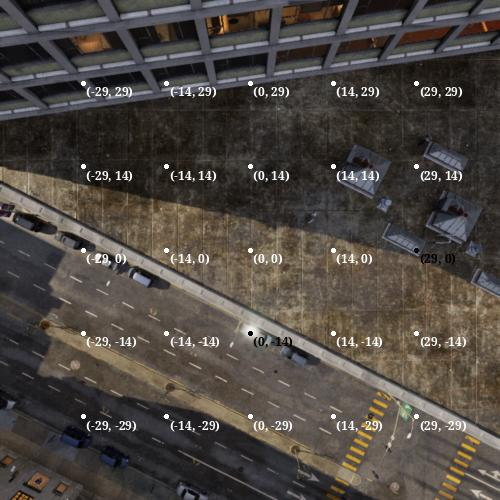
\includegraphics[width=0.5\linewidth]{images/Sonnet-CityNew-FS2/20_19.jpg}
    \end{center}
    
\gptspeaks: \( < \)Reasoning\( > \)We're getting close to our 19-move limit and haven't found the crowd yet. I notice we haven't thoroughly checked the southern area. Let's make a final move to (0, -29) and descend further to get a better view of any potential gatherings at street level.\( < \)/Reasoning\( > \)
\( < \)Action\( > \)(0, -29, -20)\( < \)/Action\( > \)
\respeaks: Your current altitude is 23 meters above ground level.
\respeaks: Image 21:
\StageDir{\re{} presents \gpt{} with a relevant image}

    \begin{center}
    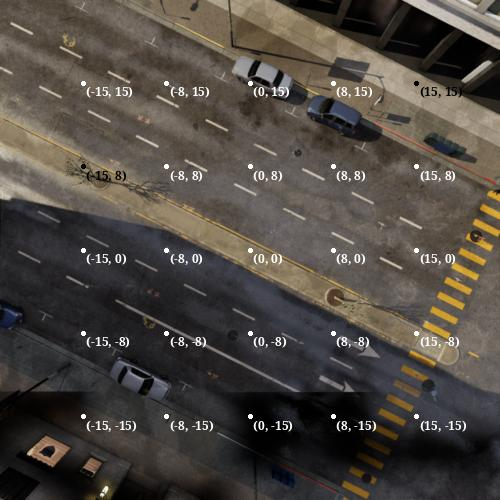
\includegraphics[width=0.5\linewidth]{images/Sonnet-CityNew-FS2/20_20.jpg}
    \end{center}
    
\gptspeaks: \( < \)Reasoning\( > \)We're now much closer to ground level but I still don't see the crowd we're looking for. With only one move left, let's check the last remaining area at (-15, 8) where there appears to be some open street space, and continue descending to get even closer to ground level.\( < \)/Reasoning\( > \)
\( < \)Action\( > \)(-15, 8, -10)\( < \)/Action\( > \)
\end{drama}
\subsubsection{Example}

    \begin{itemize}[noitemsep,topsep=0pt]
      \item Starting position: (26.0, -106.0, 118.0)
      \item End position: (98.0, -216.0, 94.0) 
      \item Euclidean distance from the object: 255.1391777050322
      \item Object can be seen: False
      \item Success: False
      \item Object type: road construction site
      
    \end{itemize}
    

    \begin{center}
    \includegraphics[width=0.7\linewidth]{images/Sonnet-CityNew-FS2/21.pdf}
    \end{center}
    

    \begin{center}
    \includegraphics[width=0.7\linewidth]{images/Sonnet-CityNew-FS2/21_sit_awareness.pdf}
    \end{center}
    

    \begin{drama}
    \Character{Benchmark}{re}
    \Character{Claude 3.5 Sonnet}{gpt}
    
\respeaks: \( < \)Context\( > \)
    You are in command of a UAV, tasked with finding road construction site.
\( < \)/Context\( > \) \texttt{(REST OF THE PROMPT)}
\respeaks: The object you're looking for is similar to this. This is NOT the drone's current view.
\respeaks: Image 1:
\StageDir{\re{} presents \gpt{} with a relevant image}

    \begin{center}
    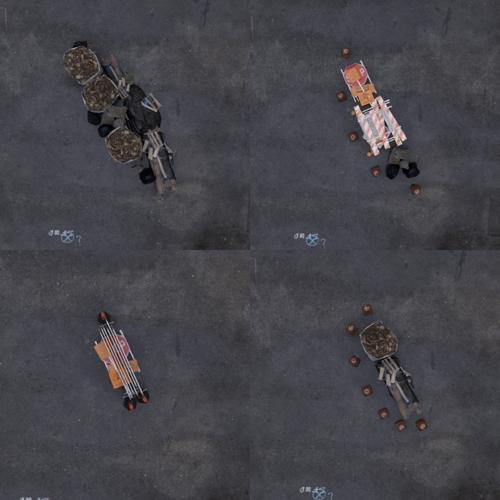
\includegraphics[width=0.5\linewidth]{images/Sonnet-CityNew-FS2/21_0.jpg}
    \end{center}
    
\respeaks: Your current altitude is 118 meters above ground level.
\respeaks: Image 2:
\StageDir{\re{} presents \gpt{} with a relevant image}

    \begin{center}
    
\includegraphics[width=0.5\linewidth]{images/Sonnet-CityNew-FS2/21_1.jpg}
    \end{center}
    
\gptspeaks: \( < \)Reasoning\( > \)From the high altitude of 118 meters, I need to conduct a systematic search for the road construction equipment. I can see several areas that need closer inspection. I'll start by moving to coordinates (39, 0) and reducing altitude by 60 meters to get a better view of the central area. This will give me a good vantage point to spot any construction equipment while maintaining enough height to keep a broad field of view.\( < \)/Reasoning\( > \)
\( < \)Action\( > \)(39, 0, -60)\( < \)/Action\( > \)
\respeaks: Your current altitude is 58 meters above ground level.
\respeaks: Image 3:
\StageDir{\re{} presents \gpt{} with a relevant image}

    \begin{center}
    
\includegraphics[width=0.5\linewidth]{images/Sonnet-CityNew-FS2/21_2.jpg}
    \end{center}
    
\gptspeaks: \( < \)Reasoning\( > \)I can see what appears to be construction equipment near coordinates (0, 0). I'll move closer to that position and reduce altitude further by 40 meters to get a better look and ensure I'm within the required 10-meter height requirement.\( < \)/Reasoning\( > \)
\( < \)Action\( > \)(0, 0, -40)\( < \)/Action\( > \)
\respeaks: Emergency stop; you've flown too close to something and would have hit it.
\respeaks: Your current altitude is 34 meters above ground level.
\respeaks: Image 4:
\StageDir{\re{} presents \gpt{} with a relevant image}

    \begin{center}
    
\includegraphics[width=0.5\linewidth]{images/Sonnet-CityNew-FS2/21_3.jpg}
    \end{center}
    
\gptspeaks: \( < \)Reasoning\( > \)I need to be more careful with my movements. I can see construction equipment near my current position, but I need to get closer while maintaining a safe distance. I'll make a smaller adjustment to my position and reduce altitude by 25 meters to get within the required 10-meter height while staying safe.\( < \)/Reasoning\( > \)
\( < \)Action\( > \)(11, 0, -25)\( < \)/Action\( > \)
\respeaks: Emergency stop; you've flown too close to something and would have hit it.
\respeaks: Your current altitude is 34 meters above ground level.
\respeaks: Image 5:
\StageDir{\re{} presents \gpt{} with a relevant image}

    \begin{center}
    
\includegraphics[width=0.5\linewidth]{images/Sonnet-CityNew-FS2/21_4.jpg}
    \end{center}
    
\gptspeaks: \( < \)Reasoning\( > \)I need to adjust my strategy. Let me try moving to a slightly different position and reduce altitude by a smaller amount to avoid any potential collisions. I'll move to (19, 11) and descend 15 meters to get a safer angle on the construction site.\( < \)/Reasoning\( > \)
\( < \)Action\( > \)(19, 11, -15)\( < \)/Action\( > \)
\respeaks: Emergency stop; you've flown too close to something and would have hit it.
\respeaks: Your current altitude is 34 meters above ground level.
\respeaks: Image 6:
\StageDir{\re{} presents \gpt{} with a relevant image}

    \begin{center}
    
\includegraphics[width=0.5\linewidth]{images/Sonnet-CityNew-FS2/21_5.jpg}
    \end{center}
    
\gptspeaks: \( < \)Reasoning\( > \)I'm having difficulty getting closer safely. Let me try moving to a position further out first and then reassess. I'll move to (23, 23) to get a different perspective while maintaining the current altitude.\( < \)/Reasoning\( > \)
\( < \)Action\( > \)(23, 23, 0)\( < \)/Action\( > \)
\respeaks: Emergency stop; you've flown too close to something and would have hit it.
\respeaks: Your current altitude is 34 meters above ground level.
\respeaks: Image 7:
\StageDir{\re{} presents \gpt{} with a relevant image}

    \begin{center}
    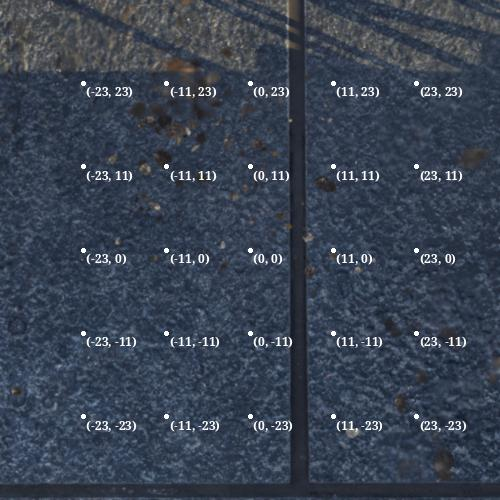
\includegraphics[width=0.5\linewidth]{images/Sonnet-CityNew-FS2/21_6.jpg}
    \end{center}
    
\gptspeaks: \( < \)Reasoning\( > \)I need to change my approach. Let me first gain some altitude to get a better overview and then plan a safer descent path. I'll move up by 20 meters first while staying in my current position.\( < \)/Reasoning\( > \)
\( < \)Action\( > \)(0, 0, 20)\( < \)/Action\( > \)
\respeaks: Your current altitude is 54 meters above ground level.
\respeaks: Image 8:
\StageDir{\re{} presents \gpt{} with a relevant image}

    \begin{center}
    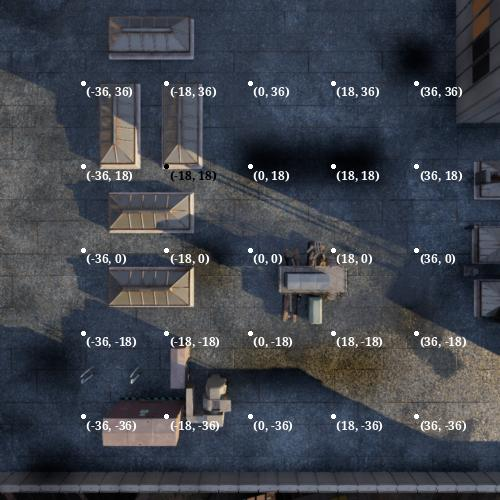
\includegraphics[width=0.5\linewidth]{images/Sonnet-CityNew-FS2/21_7.jpg}
    \end{center}
    
\gptspeaks: \( < \)Reasoning\( > \)Now I have a better view of the area. I can see the construction equipment more clearly. I'll move to (18, 0) to get a better position near the target while keeping my current altitude. This should give me a safer approach angle.\( < \)/Reasoning\( > \)
\( < \)Action\( > \)(18, 0, 0)\( < \)/Action\( > \)
\respeaks: Your current altitude is 54 meters above ground level.
\respeaks: Image 9:
\StageDir{\re{} presents \gpt{} with a relevant image}

    \begin{center}
    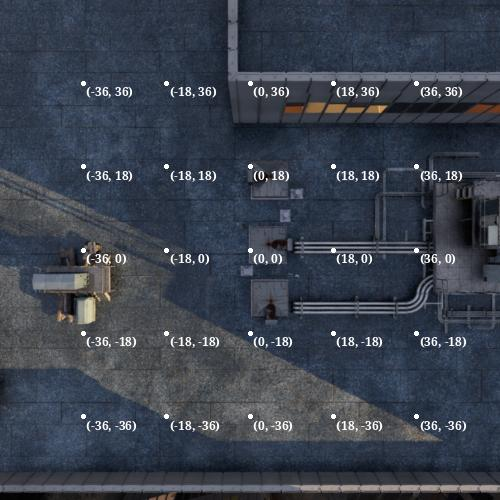
\includegraphics[width=0.5\linewidth]{images/Sonnet-CityNew-FS2/21_8.jpg}
    \end{center}
    
\gptspeaks: \( < \)Reasoning\( > \)From this position, I can see the construction equipment more clearly. I'll now try to descend gradually to get within 10 meters of it. I'll reduce altitude by 45 meters to get close to the required height while staying in the same horizontal position.\( < \)/Reasoning\( > \)
\( < \)Action\( > \)(18, 0, -45)\( < \)/Action\( > \)
\respeaks: Emergency stop; you've flown too close to something and would have hit it.
\respeaks: Your current altitude is 34 meters above ground level.
\respeaks: Image 10:
\StageDir{\re{} presents \gpt{} with a relevant image}

    \begin{center}
    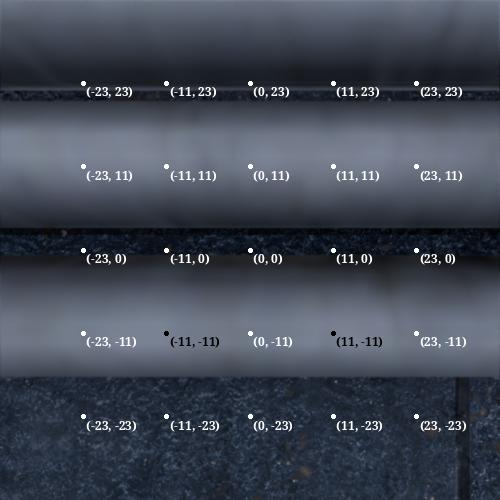
\includegraphics[width=0.5\linewidth]{images/Sonnet-CityNew-FS2/21_9.jpg}
    \end{center}
    
\gptspeaks: \( < \)Reasoning\( > \)I need to move to a position where I have better visibility and can safely descend. I'll move to (0, -23) which should give me a clearer view from a different angle while maintaining my current altitude.\( < \)/Reasoning\( > \)
\( < \)Action\( > \)(0, -23, 0)\( < \)/Action\( > \)
\respeaks: Emergency stop; you've flown too close to something and would have hit it.
\respeaks: Your current altitude is 34 meters above ground level.
\respeaks: Image 11:
\StageDir{\re{} presents \gpt{} with a relevant image}

    \begin{center}
    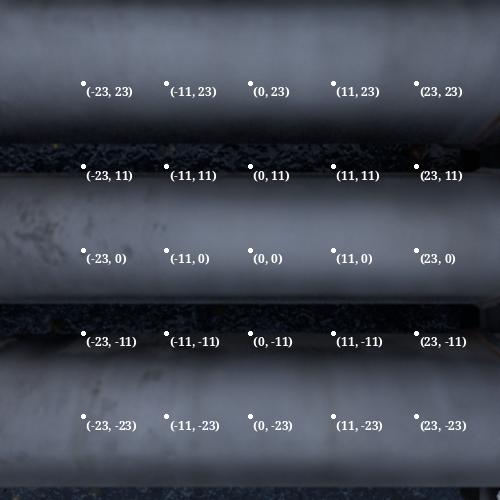
\includegraphics[width=0.5\linewidth]{images/Sonnet-CityNew-FS2/21_10.jpg}
    \end{center}
    
\gptspeaks: \( < \)Reasoning\( > \)I seem to be in a difficult position with limited visibility and movement options. Let me first gain some altitude to get a better overview of the situation. I'll move up 30 meters while staying in my current position.\( < \)/Reasoning\( > \)
\( < \)Action\( > \)(0, 0, 30)\( < \)/Action\( > \)
\respeaks: Your current altitude is 64 meters above ground level.
\respeaks: Image 12:
\StageDir{\re{} presents \gpt{} with a relevant image}

    \begin{center}
    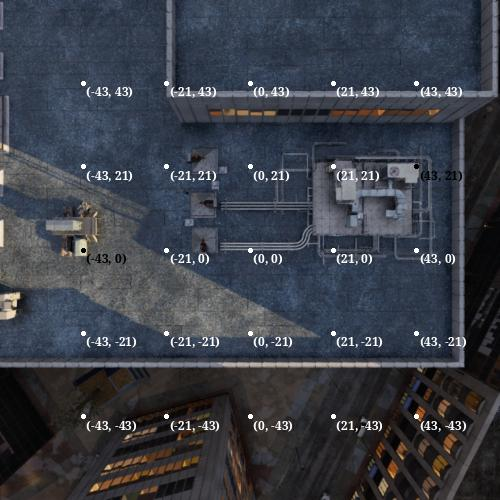
\includegraphics[width=0.5\linewidth]{images/Sonnet-CityNew-FS2/21_11.jpg}
    \end{center}
    
\gptspeaks: \( < \)Reasoning\( > \)Now I have a better view. I can see the construction equipment near (-43, 0). I'll move to that position while maintaining this safer altitude, which should give me a better approach angle for my final descent.\( < \)/Reasoning\( > \)
\( < \)Action\( > \)(-43, 0, 0)\( < \)/Action\( > \)
\respeaks: Your current altitude is 64 meters above ground level.
\respeaks: Image 13:
\StageDir{\re{} presents \gpt{} with a relevant image}

    \begin{center}
    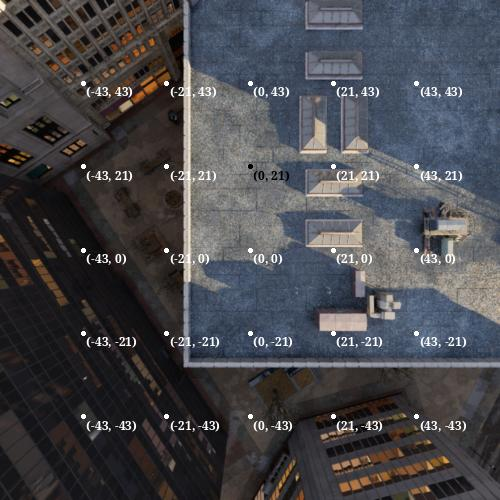
\includegraphics[width=0.5\linewidth]{images/Sonnet-CityNew-FS2/21_12.jpg}
    \end{center}
    
\gptspeaks: \( < \)Reasoning\( > \)From this position, I can see the construction site more clearly. I'll try to move to (-21, 0) which appears to be a safer position closer to the target, while maintaining my current altitude. This should give me a better vantage point for the final approach.\( < \)/Reasoning\( > \)
\( < \)Action\( > \)(-21, 0, 0)\( < \)/Action\( > \)
\respeaks: Your current altitude is 64 meters above ground level.
\respeaks: Image 14:
\StageDir{\re{} presents \gpt{} with a relevant image}

    \begin{center}
    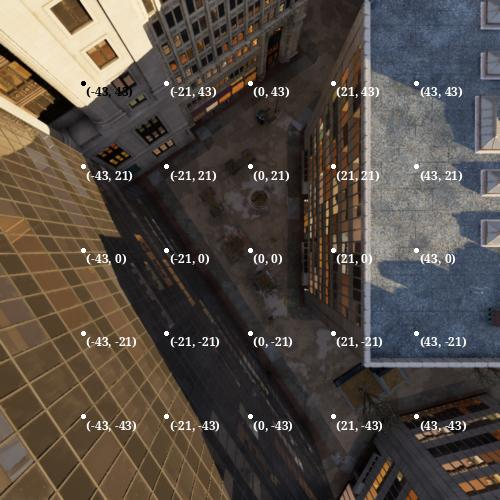
\includegraphics[width=0.5\linewidth]{images/Sonnet-CityNew-FS2/21_13.jpg}
    \end{center}
    
\gptspeaks: \( < \)Reasoning\( > \)I need to get to a position where I have a clearer view of the construction site. I'll move to (-21, -21) to get away from the buildings and have a better angle, while maintaining my current altitude.\( < \)/Reasoning\( > \)
\( < \)Action\( > \)(-21, -21, 0)\( < \)/Action\( > \)
\respeaks: Emergency stop; you've flown too close to something and would have hit it.
\respeaks: Your current altitude is 64 meters above ground level.
\respeaks: Image 15:
\StageDir{\re{} presents \gpt{} with a relevant image}

    \begin{center}
    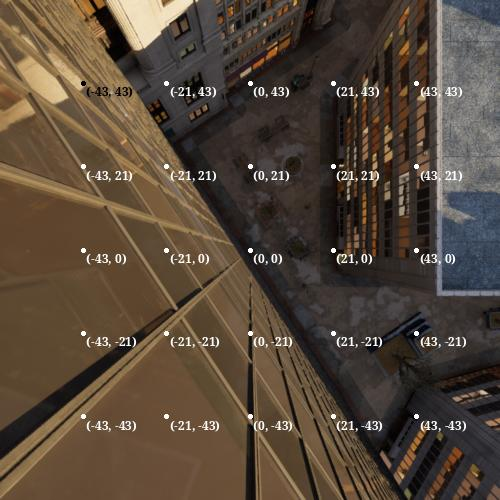
\includegraphics[width=0.5\linewidth]{images/Sonnet-CityNew-FS2/21_14.jpg}
    \end{center}
    
\gptspeaks: \( < \)Reasoning\( > \)I seem to be in a challenging position near tall buildings. I need to move to a more open area. Let me try moving to (0, 43) which should take me away from the buildings while maintaining the current altitude.\( < \)/Reasoning\( > \)
\( < \)Action\( > \)(0, 43, 0)\( < \)/Action\( > \)
\respeaks: Your current altitude is 64 meters above ground level.
\respeaks: Image 16:
\StageDir{\re{} presents \gpt{} with a relevant image}

    \begin{center}
    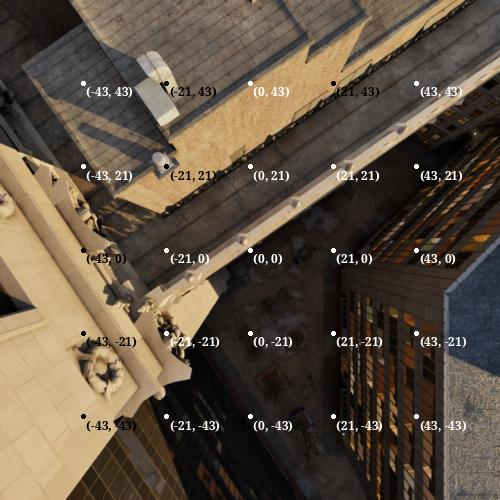
\includegraphics[width=0.5\linewidth]{images/Sonnet-CityNew-FS2/21_15.jpg}
    \end{center}
    
\gptspeaks: \( < \)Reasoning\( > \)I need to get away from these buildings and find a clearer path to the construction site. Let me move to (43, 43) which appears to be a more open area, while maintaining altitude.\( < \)/Reasoning\( > \)
\( < \)Action\( > \)(43, 43, 0)\( < \)/Action\( > \)
\respeaks: Your current altitude is 64 meters above ground level.
\respeaks: Image 17:
\StageDir{\re{} presents \gpt{} with a relevant image}

    \begin{center}
    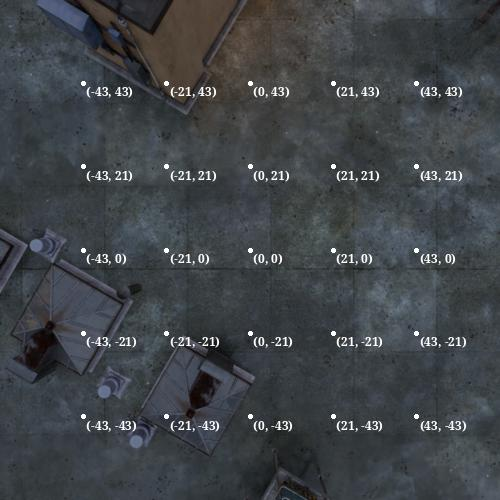
\includegraphics[width=0.5\linewidth]{images/Sonnet-CityNew-FS2/21_16.jpg}
    \end{center}
    
\gptspeaks: \( < \)Reasoning\( > \)Now I have a clearer view of the area. I'll move to (21, 21) which should give me a better position to approach the construction site area, while keeping the current altitude.\( < \)/Reasoning\( > \)
\( < \)Action\( > \)(21, 21, 0)\( < \)/Action\( > \)
\respeaks: Emergency stop; you've flown too close to something and would have hit it.
\respeaks: Your current altitude is 64 meters above ground level.
\respeaks: Image 18:
\StageDir{\re{} presents \gpt{} with a relevant image}

    \begin{center}
    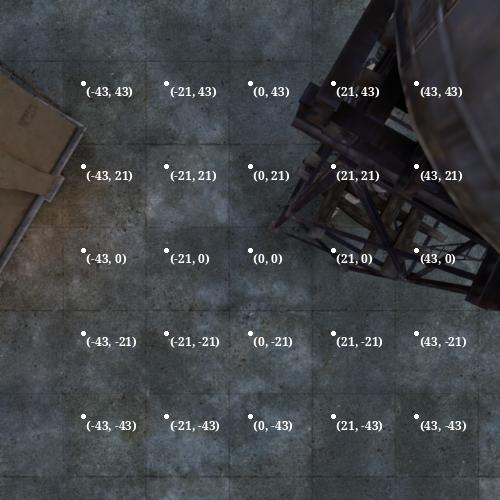
\includegraphics[width=0.5\linewidth]{images/Sonnet-CityNew-FS2/21_17.jpg}
    \end{center}
    
\gptspeaks: \( < \)Reasoning\( > \)I'm still encountering obstacles. Let me try moving to (0, 21) which should be a clearer path while maintaining the current altitude. This position might give me a better angle to approach the target area.\( < \)/Reasoning\( > \)
\( < \)Action\( > \)(0, 21, 0)\( < \)/Action\( > \)
\respeaks: Emergency stop; you've flown too close to something and would have hit it.
\respeaks: Your current altitude is 64 meters above ground level.
\respeaks: Image 19:
\StageDir{\re{} presents \gpt{} with a relevant image}

    \begin{center}
    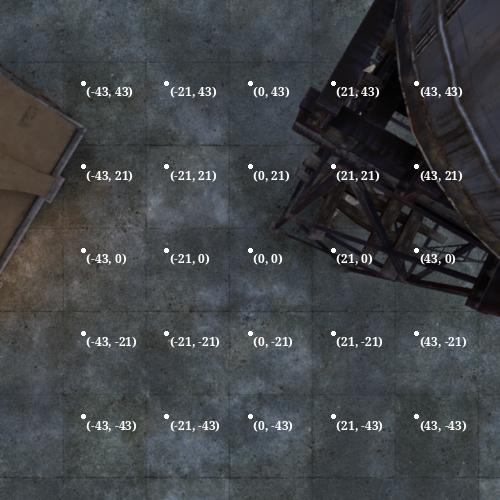
\includegraphics[width=0.5\linewidth]{images/Sonnet-CityNew-FS2/21_18.jpg}
    \end{center}
    
\gptspeaks: \( < \)Reasoning\( > \)I need to try a different strategy. Let me first gain more altitude to get a better overview and avoid obstacles. I'll increase height by 30 meters while staying in my current position.\( < \)/Reasoning\( > \)
\( < \)Action\( > \)(0, 0, 30)\( < \)/Action\( > \)
\respeaks: Your current altitude is 94 meters above ground level.
\respeaks: Image 20:
\StageDir{\re{} presents \gpt{} with a relevant image}

    \begin{center}
    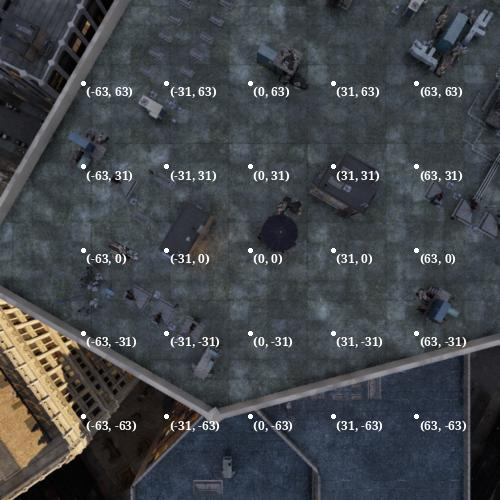
\includegraphics[width=0.5\linewidth]{images/Sonnet-CityNew-FS2/21_19.jpg}
    \end{center}
    
\gptspeaks: \( < \)Reasoning\( > \)From this higher altitude, I have a better view of the area. I can see the road and various structures more clearly. I'll move to (31, 31) which appears to be a clearer area while maintaining this altitude, and then I can plan a safer descent path.\( < \)/Reasoning\( > \)
\( < \)Action\( > \)(31, 31, 0)\( < \)/Action\( > \)
\respeaks: Your current altitude is 94 meters above ground level.
\respeaks: Image 21:
\StageDir{\re{} presents \gpt{} with a relevant image}

    \begin{center}
    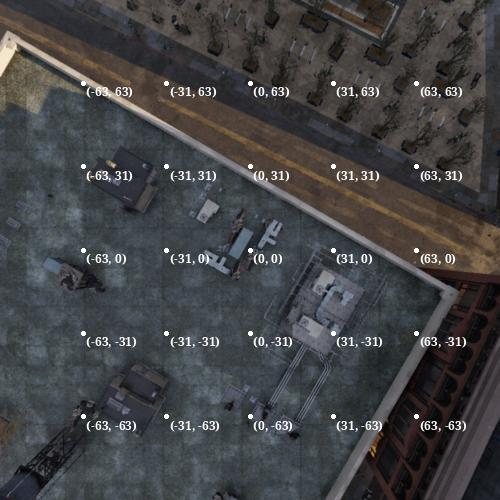
\includegraphics[width=0.5\linewidth]{images/Sonnet-CityNew-FS2/21_20.jpg}
    \end{center}
    
\gptspeaks: \( < \)Reasoning\( > \)I can see more of the area now. I'll move to (-31, 0) to get closer to where I saw the construction equipment earlier, while maintaining this safer altitude before attempting a final approach.\( < \)/Reasoning\( > \)
\( < \)Action\( > \)(-31, 0, 0)\( < \)/Action\( > \)
\end{drama}
